\documentclass{article}
    % General document formatting
    \usepackage[margin=0.7in]{geometry}
    \usepackage[parfill]{parskip}
    \usepackage[utf8]{inputenc}
    
    % Related to math
    \usepackage{amsmath,amssymb,amsfonts,amsthm}
\usepackage{graphicx}
%\usepackage{subfig}
%\usepackage{subfigure}
\usepackage{caption}
\usepackage{subcaption}
\usepackage{listings}
\usepackage[percent]{overpic}
\usepackage{xcolor,varwidth}

\usepackage{titling}
%\usepackage{lipsum}

\usepackage{titlesec}

\titleformat*{\section}{\Large\bfseries}
\titleformat*{\subsection}{\large\bfseries}
%\titleformat*{\subsubsection}{\large\bfseries}
%\titleformat*{\paragraph}{\large\bfseries}
%\titleformat*{\subparagraph}{\large\bfseries}
\titlespacing\section{0pt}{12pt plus 4pt minus 2pt}{0pt plus 2pt minus 2pt}
\titlespacing\subsection{0pt}{12pt plus 4pt minus 2pt}{0pt plus 2pt minus 2pt}
\titlespacing\subsubsection{0pt}{12pt plus 4pt minus 2pt}{0pt plus 2pt minus 2pt}

\pretitle{\begin{center}\large\bfseries}
\posttitle{\par\end{center}\vskip 0.01em}
\preauthor{\begin{center}\Large\ttfamily}
\postauthor{\end{center}}
\predate{\par\normalsize\centering}
\postdate{\par}

\title{Population Genetic Analyses of Genomic Data 1}
%\date{\today}


\begin{document}

%\maketitle

\begin{center}
%\textbf{\LARGE{\centering{A simple CX firing rate model}}}\\
%\textit{USN: 303039534}\\
\end{center}

%\normalsize{   }
%~\\


\section{Structure and equations}

take home messages: we do not need the smoothening with von Mises functions to get accurate integration; this can be achieved with 8 discrete EPG neurons. The real connectivity also includes neighboring connections which could also be implemented.

What is PEG-EPG connectivity if there is any? Gap junctions, via PEN2s?

\begin{equation}
f(x) = tanh(x)
\end{equation}

\begin{equation}
\tau_{EPG} \dfrac{dEPG}{dt} = -EPG + f(W_{PEG,EPG}\cdot PEG + W_{PEN1_L,EPG}\cdot PEN1_L + W_{PEN1_R,EPG}\cdot PEN1_R + W_{EPG,EPG}\cdot EPG)
\end{equation}

\begin{equation}
\tau_{PEG} \dfrac{dPEG}{dt} = -PEG + f(W_{EPG,PEG}\cdot EPG - W_{D7,PEG}\cdot D7 )
\end{equation}

\begin{equation}
\tau_{D7} \dfrac{dD7}{dt} =-D7 + f(W_{EPG,D7}\cdot EPG)
\end{equation}

\begin{equation}
\tau_{PEN1} \dfrac{dPEN1_L}{dt} = -PEN1_L + f(W_{EPG,PEN1_L}\cdot EPG - W_{D7,PEN1_L}\cdot D7 + v_L )
\end{equation}

\begin{equation}
\tau_{PEN1} \dfrac{dPEN1_R}{dt} = -PEN1_R + f(W_{EPG,PEN1_R}\cdot EPG - W_{D7,PEN1_R}\cdot D7 + v_R )
\end{equation}

constraining all firing rates to be positive.



\section{Integrating velocities}


\begin{figure}[h]
	\centering
	\begin{subfigure}[t]{0.43\linewidth}
		\centering
		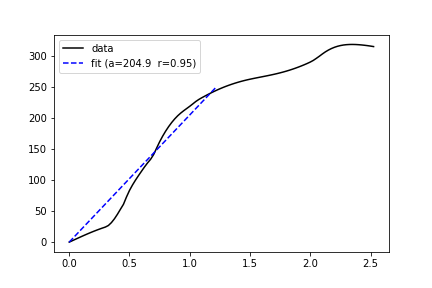
\includegraphics[width = 1.0\linewidth, trim={0 0 0 0}, clip=true]{../figures/testvels_early.png}
		\subcaption{equilibrate for 1000 ms, measure mean veocity over 500 ms -> early velocity}
		\label{fig:F}	
	\end{subfigure}
	\hspace{0.1\linewidth}
	\begin{subfigure}[t]{0.43\linewidth}
		\centering
		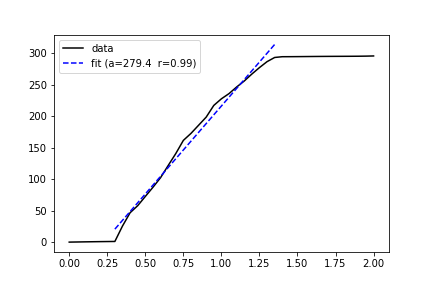
\includegraphics[width = 1.0\linewidth, trim={0 0 0 0}, clip=true]{../figures/testvels_late.png}
		\caption{For small input, turning is not sustained. Can instead equilibrate for 1000ms, run for 9000 ms.}
		\label{fig:dF}
	\end{subfigure}
\caption{}
\label{fig:fit}
\end{figure}

1. equilibrate for 1000 ms, measure mean veocity over 500 ms - early velocity

2. at low angular velocities, this does not lead to a full bump shift and turning is not sustained -> mean velocity at later period

\section{tracking experimental data}

\begin{figure}[h]
	\centering
	\begin{subfigure}[t]{0.43\linewidth}
		\centering
		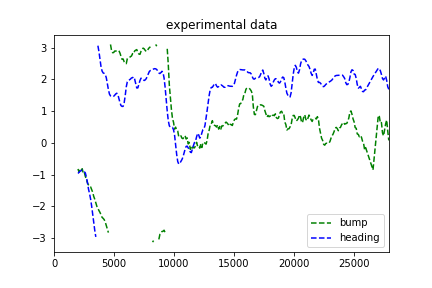
\includegraphics[width = 1.0\linewidth, trim={0 0 0 0}, clip=true]{../figures/real_heading.png}
		\subcaption{real heading and bump position}
		\label{fig:F}	
	\end{subfigure}
	\hspace{0.1\linewidth}
	\begin{subfigure}[t]{0.43\linewidth}
		\centering
		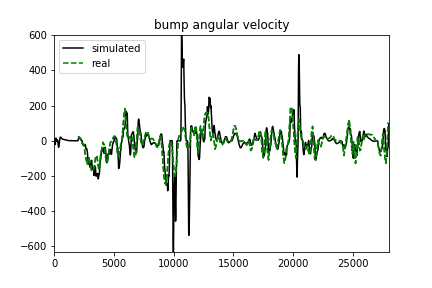
\includegraphics[width = 1.0\linewidth, trim={0 0 0 0}, clip=true]{../figures/sim_vel.png}
		\caption{real and simulated velocity curves}
		\label{fig:dF}
	\end{subfigure}
\caption{}
\label{fig:fit}
\end{figure}

\begin{figure}[h]
	\centering
	\begin{subfigure}[t]{0.73\linewidth}
		\centering
		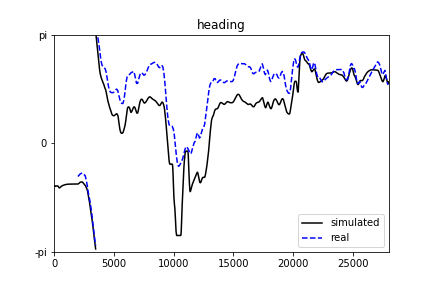
\includegraphics[width = 1.0\linewidth, trim={0 0 0 0}, clip=true]{../figures/sim_head.png}
		\subcaption{real heading and simulated bump}
		\label{fig:F}	
	\end{subfigure}
	\hspace{0.1\linewidth}
	\begin{subfigure}[t]{0.73\linewidth}
		\centering
		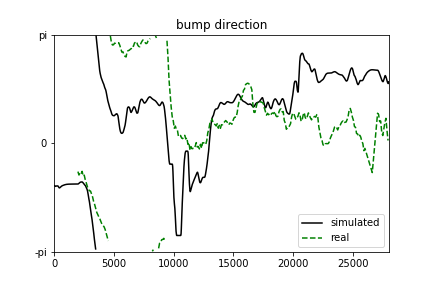
\includegraphics[width = 1.0\linewidth, trim={0 0 0 0}, clip=true]{../figures/sim_bump.png}
		\caption{real bump and simulated bump}
		\label{fig:dF}
	\end{subfigure}
\caption{}
\label{fig:fit}
\end{figure}

We see that our integrator does not quite follow the long rapid turn; but neither does the real bump (right) which actually does a worse job recovering from the turn.

The poor performance can result from very rapid turns leading to strong global PEN1 and thus EPG excitation, which in turn mediates D7 excitation and global inhibition. Thus broad excitation leads to downstream global inhibition and quenching of the bump. This is different from the real system where the bump intensity tends to correlate positively with rotational velocity...
Local recurrence EPG - EPG in the EB helos prevent this by retaining activity during strong inhibition of PEN1 and PEG.


\begin{figure}[h]
	\centering
	\begin{subfigure}[t]{0.73\linewidth}
		\centering
		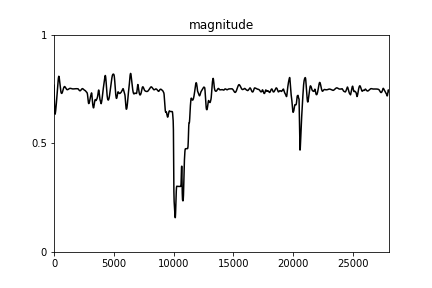
\includegraphics[width = 1.0\linewidth, trim={0 0 0 0}, clip=true]{../figures/sim_mag.png}
		\subcaption{magnitude of PVA average. This decreases strongly near the rapid turn at 10000 ms}
		\label{fig:F}	
	\end{subfigure}
	\hspace{0.1\linewidth}
	\begin{subfigure}[t]{0.73\linewidth}
		\centering
		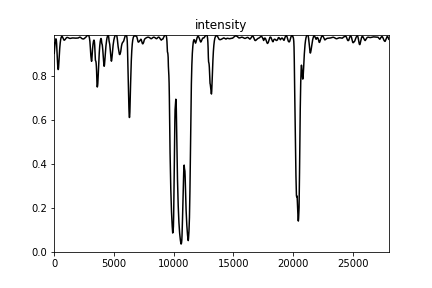
\includegraphics[width = 1.0\linewidth, trim={0 0 0 0}, clip=true]{../figures/sim_int.png}
		\caption{intensity of the most active EPG neuron (bump height). This decreases strongly following global inhibition near the rapid turn at 1000 ms.}
		\label{fig:dF}
	\end{subfigure}
\caption{}
\label{fig:fit}
\end{figure}

Also note intensity and magnitude oscillates at steady state - do we observe this in the data? general feature that dynamical systems can react to changes faster than static systems (metabolism, tennis serve etc...)

\section{Simulating shibire experiments}

\begin{figure}[h]
	\centering
	\begin{subfigure}[t]{0.73\linewidth}
		\centering
		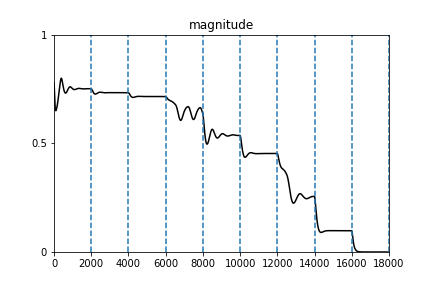
\includegraphics[width = 1.0\linewidth, trim={0 0 0 0}, clip=true]{../figures/D7_sequential_mags.png}
		\subcaption{magnitude of PVA average  for sequential shibire inhition (0, 10\%, 20\%, ...).}
		\label{fig:F}	
	\end{subfigure}
	\hspace{0.1\linewidth}
%	\begin{subfigure}[t]{0.73\linewidth}
%		\centering
%		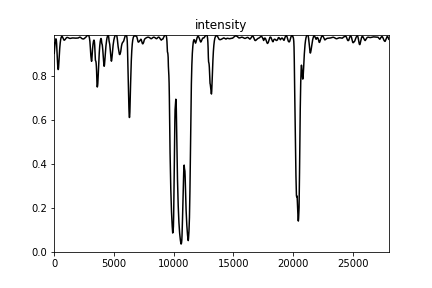
\includegraphics[width = 1.0\linewidth, trim={0 0 0 0}, clip=true]{../figures/sim_int.png}
%		\caption{intensity of the most active EPG neuron (bump height). This decreases strongly following global inhibition near the rapid turn at 1000 ms.}
%		\label{fig:dF}
%	\end{subfigure}
\caption{}
\label{fig:fit}
\end{figure}


\begin{figure}[h]
	\centering
	\begin{subfigure}[t]{0.32\linewidth}
		\centering
		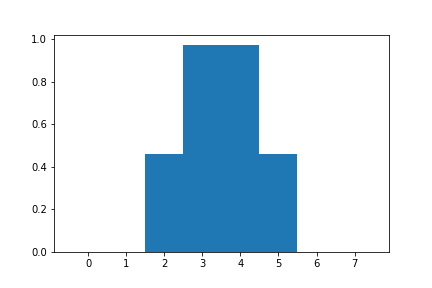
\includegraphics[width = 1.0\linewidth, trim={20 20 20 20}, clip=true]{../figures/D7_inhib_10.png}
		\subcaption{No inhibition}
		\label{fig:F}	
	\end{subfigure}
	\hspace{0.001\linewidth}
	\begin{subfigure}[t]{0.32\linewidth}
		\centering
		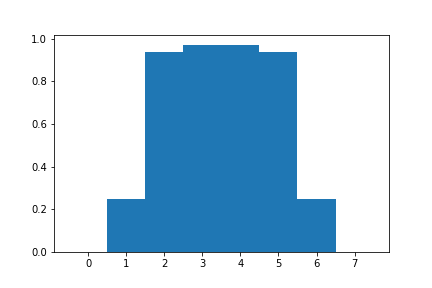
\includegraphics[width = 1.0\linewidth, trim={20 20 20 20}, clip=true]{../figures/D7_inhib_06.png}
		\caption{30\% inhibition}
		\label{fig:dF}
	\end{subfigure}
	\hspace{0.001\linewidth}
	\begin{subfigure}[t]{0.32\linewidth}
		\centering
		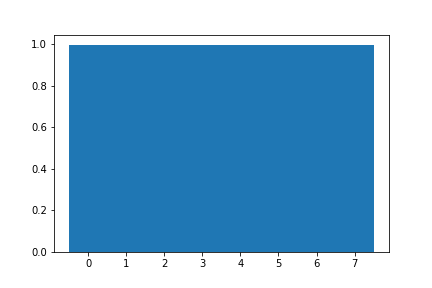
\includegraphics[width = 1.0\linewidth, trim={20 20 20 20}, clip=true]{../figures/D7_inhib_03.png}
		\caption{70\% inhibition}
		\label{fig:dF}
	\end{subfigure}
\caption{}
\label{fig:fit}
\end{figure}

\begin{figure}[h]
	\centering
	\begin{subfigure}[t]{0.48\linewidth}
		\centering
		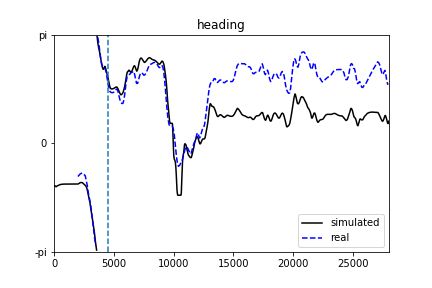
\includegraphics[width = 1.0\linewidth, trim={0 0 0 0}, clip=true]{../figures/sim_head_D7_07.png}
		\subcaption{30\% inhibition}
		\label{fig:F}	
	\end{subfigure}
	\hspace{0.01\linewidth}
	\begin{subfigure}[t]{0.48\linewidth}
		\centering
		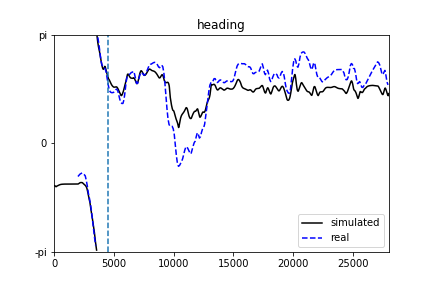
\includegraphics[width = 1.0\linewidth, trim={0 0 0 0}, clip=true]{../figures/sim_head_D7_04.png}
		\caption{60\% inhibition}
		\label{fig:dF}
	\end{subfigure}
\caption{vertical line indicates time of inhibition.}
\label{fig:fit}
\end{figure}

\begin{figure}[h]
	\centering
	\begin{subfigure}[t]{0.48\linewidth}
		\centering
		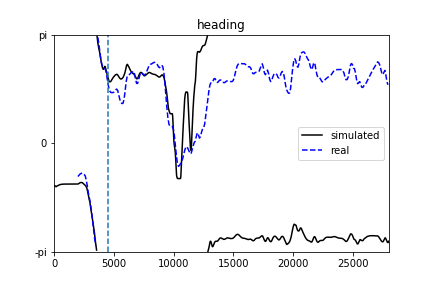
\includegraphics[width = 1.0\linewidth, trim={0 0 0 0}, clip=true]{../figures/sim_head_PEN1_07.png}
		\subcaption{30\% inhibition PEN1}
		\label{fig:F}	
	\end{subfigure}
	\hspace{0.01\linewidth}
	\begin{subfigure}[t]{0.48\linewidth}
		\centering
		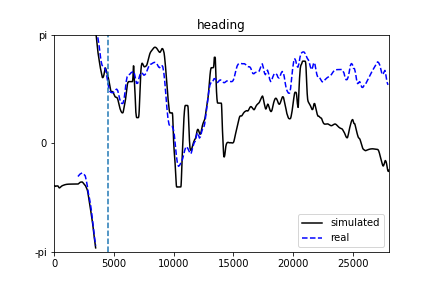
\includegraphics[width = 1.0\linewidth, trim={0 0 0 0}, clip=true]{../figures/sim_head_PEG_07.png}
		\caption{30\% inhibition PEG}
		\label{fig:dF}
	\end{subfigure}
\caption{vertical line indicates time of inhibition.}
\label{fig:fit}
\end{figure}


\end{document}

\subsection{Measurement of variance}

\begin{table}[h]
\centering
\begin{tabular}{ |c|c|c|c|}
\hline
 & Sample size & Allele frequency \\
\hline
Selected population & 124 & 0.43 \\
\hline
Unselected population & 176 & 0.34 \\
\hline
\end{tabular}
\caption{Collected data}
\label{tab:data}
\end{table}

\textbf{a)}
Given the data in table \ref{tab:data} for allele frequencies of A in insects treated or untreated with a mild insectiside, we can calculate $F_{ST}$, quantifying the difference in degree of heterozygosity between the two populations.
From the definition of $F_{ST}$, we have:
\begin{equation}
F_{ST} = 1 - \dfrac{2q_A^Sq_a^S}{2q_A^Tq_a^T} = 
1 - \dfrac{ N^{S_1}q_A^{S_1}q_a^{S_1} + N^{S_2}q_A^{S_2}q_a^{S_2}}{q_A^Tq_a^T(N^{S_1}+N^{S_2})}
\end{equation}
Inserting the data from table \ref{tab:data} gives
\begin{equation*}
F_{ST} = 1- \dfrac{124*0.43*0.57 + 176*0.34*0.66}{ \dfrac{124*0.43+176*0.34}{300} * \dfrac{124*0.57+176*0.66}{300}*300 }
= 0.008361 = 0.836 \%
\end{equation*}

The fixation index $F_{ST}$ is thus \textbf{0.008361}.

\textbf{b)}
We assume that the two subpopulations are both large enough to ignore genetic drift and that the 'selected population' is the population treated with insecticide. Now if I were to conduct a statistical test and it showed $F_{ST}$ to be significantly greater than zero, I would conclude that treatment with insecticide is likely to enrich for the measured allele in the insect population. This could have one of a number of different causes. The simplest is that the measured allele confers an evolutionary advantage in the presence of the insecticide, leading to direct selection for this allele in the presence but not the absence of insecticide, and hence the observed difference in heterozygosity suggested by $F_{ST} > 0$. An alternative explanation is that the locus of interest is genetically linked to a gene or genomic region that confers a selective advantage/disadvantage in the presence of the insecticide.


\subsection{Modelling fitness in a diploid system}

We now consider a set of diploid organisms with a fraction $p_i$ infected by a parasite. Consider allele A at locus A/a to have frequency $p$ and allele a at the same locus to have an allele frequency of $q = 1-p$. We further specify that the fitness (here given as the 'growth rate' of the organism) is dependent on infection state and genetic composition at locus A/a as given by table \ref{tab:fitness}

\begin{table}[h]
\centering
\begin{tabular}{ |c|c|c|c|}
\hline
 & AA & Aa & aa \\
\hline
Infected & a & b & c \\
Not infected & 1 &1 & c\\
\hline
\end{tabular}
\caption{Fitness of individuals}
\label{tab:fitness}
\end{table}

Here, $a, b, c \in \, ]0, 1[$

\textbf{a)}
The Hardy-Weinberg proportions specify the relative proportion of organisms with each genotype that would lead to a stable equilibrium given the allele frequencies. This is given by

$f(AA) = p^2$\\
$f(Aa) = pq + qp = 2pq$\\
$f(aa) = q^2$\\

This can be visualized as the relative areas of the diagonal and off-diagonal sections of the population Punnett square.

\textbf{b)}
We now assume the following values:\\
$p=0.5\\ q=1-p=0.5\\ a=0.8\\ b=0.9\\ c=0.7\\ p_i = 0.9$\\
This allows us to calculate the mean fitness of the population as the weighted mean of the fitnesses of the infected and uninfected populations. We denote the fitness $F$ with subscripts i and u to denote infected and uninfected subpopulations. $F_m$ denotes the mean fitness.
\begin{equation*}
F_{m} = p_i * ( f(AA) * F_i(AA) + f(Aa) * F_i(Aa) + f(aa) * F_i(aa) ) + (1-p_i )* (f(AA) * F_u(AA) + f(Aa) * F_u(Aa) + f(aa) * F_u(aa))
\end{equation*}

\begin{equation}
F_{m} = p_i * ( p^2 * a +2pq * b + q^2 * c ) + (1-p_i )* (p^2 + 2pq +q^2 * c)
\end{equation}

\begin{equation*}
F_{m} = 0.9 * ( 0.5^2 * 0.8 +2*0.5^2 * 0.9 + 0.5^2 * 0.7 ) + 0.1 * (0.5^2 + 2*0.5^2 +0.5^2 * 0.7) = 0.835
\end{equation*}

The mean fitness of the population given the specified parameters is thus \textbf{0.835}.

\textbf{c)}

We assume that the population remains in Hardy-Weinberg equilibrium. To find the value of $p$ that leads to maximum fitness while fixing the remaining parameters, we start by plotting the mean fitness of the population against the allele fraction $p$ for these values of $a$, $b$, $c$ \& $p_i$ in figure \ref{fig:F}. We see that the mean fitness has a maximum somewhere between p=0.6 and p=0.8.

\begin{figure}[h]
	\centering
	\begin{subfigure}[t]{0.43\linewidth}
		\centering
		\includegraphics[width = 1.0\linewidth, trim={0 0 0 0}, clip=true]{fitness.png}
		\subcaption{Plot of mean fitness against allele frequency $p$}
		\label{fig:F}	
	\end{subfigure}
	\hspace{0.1\linewidth}
	\begin{subfigure}[t]{0.43\linewidth}
		\centering
		\includegraphics[width = 1.0\linewidth, trim={0 0 0 0}, clip=true]{dfitness.png}
		\caption{$\dfrac{dF_{m}}{dp}$ against allele frequency $p$}
		\label{fig:dF}
	\end{subfigure}
\caption{}
\label{fig:fit}
\end{figure}

We can find the optimum value of p analytically by solving

\begin{equation*}
\dfrac{dF_{m}}{dp} = 0
\end{equation*}

This gives

\begin{equation}
\dfrac{d}{dp}[ p_i * ( p^2 * a +2(p-p^2) * b + (p^2+1-2p) * c ) + (1-p_i )* (p^2 + 2(p-p^2) +(p^2+1-2p) * c) ]= 0
\end{equation}

Evaluating the derivatives and inserting the parameter values specified in the question, we find

\begin{equation*}
 0.9 * ( 2*p * 0.8 +2(1-2*p) * 0.9 + (2*p-2) * 0.7 ) + 0.1 * (2*p + 2(1-2*p) +(2*p-2) * 0.7) = 0
\end{equation*}
\begin{equation*}
p(2*0.9*0.8-4*0.9*0.9+2*0.9*0.7+2*0.1-4*0.1+2*0.1*0.7) + (2*0.9*0.9-2*0.9*0.7+2*0.1-2*0.1*0.7) = 0
\end{equation*}

This yields an optimum allele frequency of $p = 0.7$ as expected from figure \ref{fig:fit}.
We thus see that we optimize the mean fitness of a population in Hardy-Weinberg equilibrium with $p = 0.7$ with a quadratic decrease in fitness on either side of this optimum value.

\textbf{d)}

To find the values of $b$ for which allele a is maintained in the population over long timescales, we start by plotting the mean population fitness as a function of both p and b for the values of $a$, $c$ \& $p_i$ specified in the question (figure \ref{fig:fsurf}).

\begin{figure}[h]
\centering
\includegraphics[width = 0.85\linewidth, trim={60 25 60 40}, clip=true]{fsurf.png}
\caption{Mean fitness as a function of allele frequency $p$ and infected heterozygotic fitness $F_i(Aa) = b$ }
\label{fig:fsurf}
\end{figure}

We assume a population in the limit of large size where genetic drift can be neglected.
In order to maintain the allele a in the population over long timescales, we require that the maximum mean fitness of a population in Hardy-Weinberg equilibrium occurs at $ p < 1$ for a given b. We thus return to equation (3) and write $\dfrac{\partial F_m}{\partial p}$ as a function of $b$ and $p$.

\begin{equation*}
\dfrac{\partial F_m}{\partial p} = p(2*0.9*0.8-4*0.9*b+2*0.9*0.7+2*0.1-4*0.1+2*0.1*0.7) + (2*0.9*b-2*0.9*0.7+2*0.1-2*0.1*0.7)
\end{equation*}
\begin{equation}
\dfrac{\partial F_m}{\partial p} = -3.6bp + 2.64p + 1.8b -1.2 = (2.64-3.6b) p +(1.8b-1.2)
\end{equation}

We find an extremum in p when this expression is zero, implying
\begin{equation*}
p= \dfrac{1.2 - 1.8b}{2.64 - 3.6 b}
\end{equation*}

We require this extremum to fall in $0 \leq p \leq 1$ for a local extremum within the given parameter space, and therefore find the limiting b values of biologically meaningful solutions as

\begin{equation*}
1 = \dfrac{1.2 - 1.8b}{2.64 - 3.6 b} => b = 0.8
\end{equation*}
\begin{equation*}
0 = \dfrac{1.2 - 1.8b}{2.64 - 3.6 b} => b = 0.67
\end{equation*}

Thus for $ b > 0.8 $ we have a maximum in p in the mean fitness landscape at $p<1$ (figure \ref{fig:fsurf}), giving us a non-zero frequency of the a allele at long timescales. For $b < 0.67$, we have a minimum in the fitness landscape which we will discuss further below.

We now consider the case where $0.67 < b < 0.8 $, for which there is no local extremum in p since $\dfrac{\partial F_m}{\partial p} = 0$ has no solutions for $0 \leq p \leq 1$ in this range. Setting p = 0.5, equation (4) gives us 

\begin{equation*}
\dfrac{\partial F_m}{\partial p} = -1.8b + 1.32 + 1.8b -1.2 = 0.12 > 0
\end{equation*}

Since we do not cross a point at which $\dfrac{\partial F_m}{\partial p} = 0$ for $0.67 < b < 0.8 $, $F_{m}$ must therefore be a monotonously increasing function of $p$ in this range, and the equilibrium population composition contains only AA individuals, irrespective of the initial composition of the population. In this case, the a allele is not maintained over long timescales.

We can understand the above results in a more biological context by considering the relative fitness of different individuals for various values of b.
The mean fitness of individuals with genotype AA is\\
$F_m(AA) = p_i*a + (1-p_i)*1 = 0.9*a + 0.1*1 = 0.82$\\
Similarly,\\
$F_m(Aa) = 0.9*b+0.1$\\
$F_m(aa) = 0.9*c + 0.1 * c= 0.7$\\

This is consistent with $F_{m}$ being invariant of b at p=0 where we only have aa individuals giving $F_{m} = 0.7$, and at p=1 where we only have AA individuals giving $F_{m} = 0.82$ (figure \ref{fig:fsurf}).

Since AA individuals are always more fit than aa individuals, we retain a in the population over long timescales when $F_m(Aa) > F_m(AA) $ which requires $b > \dfrac{0.82-0.1}{0.9} = 0.8$. I.e. we retain a in the population when $b > a$ since this implies that heterozygous individuals are more fit than either homozygote for the infected subpopulation, and equally fit to AA individuals in the non-infected subpopulation. This is consistent with our result above.

However, we also note that in the case of $F_m(Aa) < F_m(aa) $, we observe a local minimum in $F_{m}$ as a function of p, since starting from a population of aa individuals, introducing heterozygotes reduces the mean fitness. $F_m(Aa) < F_m(aa) $ corresponds to $b < \dfrac{0.7-0.1}{0.9} = 0.67$, again consistent with our result above. In this case, the genetic makeup of the population at long timescales depends on the initial population composition since evolution in a large population can be modeled as a steepest ascent process in $p$. If $p_{init}$ is small enough, the population will therefore move towards all individuals having the aa genotype, whereas if $p_{init}$ is large, the population will move towards all individuals being AA.

As before, the cutoff for these two scenarios is given by 
\begin{equation*}
p= \dfrac{1.2 - 1.8b}{2.64 - 3.6 b}
\end{equation*}
This allows us to predict for any value of $b$ and initial allele frequency $p_{init}$, what the long term allele frequency $p_{eq}$ will be in the limit of an infinitely large population. This can be summarized as follows: 

\begin{enumerate}

\item
$b<0.67$ and $p_{init} < \dfrac{1.2 - 1.8b}{2.64 - 3.6 b}$: The population will go to only aa individuals (the a allele \textit{is} maintained over a long period of time)

\item
$b<0.67$ and $p_{init} > \dfrac{1.2 - 1.8b}{2.64 - 3.6 b}$: The population will go to only AA individuals (the a allele \textit{is not} maintained over a long period of time)

\item
$0.67 < b < 0.80$: The population will go to only AA individuals (the a allele \textit{is not} maintained over a long period of time)

\item
$b>0.80$: The population will go to a mixture of AA, Aa and aa individuals specified by $p_{eq} = \dfrac{1.2 - 1.8b}{2.64 - 3.6 b}$ (the a allele \textit{is} maintained over a long period of time)

\end{enumerate}

This is illustrated graphically in figure \ref{fig:fsurfinit} where the z-axis represents the mean fitness for a given $b$ and $p$ while the color scheme reflects the long-term allele frequency $p_{eq}$ for a given $b$ and $p_{init}$.

\begin{figure}[h]
\centering
\begin{overpic}[width = 0.7\linewidth, trim={35 0 0 10}, clip=true]{fsurfinit.png}
%\includegraphics[width = 0.7\linewidth, trim={35 0 0 10}, clip=true]{fsurfinit.png}
\put(70,45){\color{black} \large \textit{\textbf{$F_m(b, p)$}}}
\put(100,32){\color{black} \LARGE \textit{\textbf{$p_{eq}$}}}
\end{overpic}
\caption{Plot of mean fitness (z-axis) against allele frequency $p$ and infected heterozygotic fitness $F_i(Aa) = b$. The colour scheme represents the equilibirum composition $p_{eq}$ that will be achieved over a long period of time if the population starts at a given  initial point on the fitness landscape. This corresponds to the result of a steepest ascent search along the $p$ axis. Black regions indicate initial points from which allele a \textit{is not} maintained over a long period of time ($p_{eq} = 1$). White regions indicate initial points from which allele A is not maintained ($p_{eq} = 0$). Grey regions indicate initial points from which both alleles are maintained ($0 < p_{eq} < 1$).}
\label{fig:fsurfinit}
\end{figure}

\subsection{Identifying beneficial mutations in a neutral marker experiment}

\textbf{a)} Optimist has been installed and compiled as instructed

\textbf{b)}
For the data in Colour\_freq.out when running 10 optimizations for a single mutation, every optimization gives a maximum log likelihood of $L = -92.5714$. The parameter space thus seems to be relatively well behaved as the algorithm consistently converges to the same maximum. The optimization yields a haplotype fitness of 0.049169, establishment time of 86.623 and initial frequencies of 0.359 and 0.641.

\textbf{c)}
The systematic search in discrete time yields a maximum log likelihood of -92.5725 with haplotype fitness 0.0492702, dicrete establishment time 87 and initial frequencies of 0.359 and 0.641. We thus see that this only yields a slight change in parameters from the initial optimization, with a slightly worse log likelihood due to being restricted to discrete establishment times.

We plot the model population composition together with the experimental frequencies in figure \ref{fig:mut1_s} and see that while they largely agree on the population evolution, the model fails to take into account the variation in frequencies prior to $t=87$ when the mutation is introduced.

\begin{figure}[h]
\centering
\includegraphics[width = 0.5\linewidth, trim={15 0 35 30}, clip=true]{fit_mut1.png}
\caption{Plot of model (line) and real (crosses) population compositions at different generation times. Blue vertical line indicates $t=87$ when a beneficial mutation arises in population 1.}
\label{fig:mut1_s}
\end{figure}

\newpage

\textbf{d)}

For two and three mutations, the parameter landscape in the initial optimization is less well-behaved, and we converge to maximum likelihoods ranging from -81.7427 to -81.7881 for 2 mutations and -81.1044 to -90.195 for three mutations. Running subsequent systematic optimizations on the best intial optimizations, we get the parameters specified in table \ref{tab:fitness}.

\begin{table}[h]
\centering
\begin{tabular}{ |c|c|c|c|}
\hline
 & 1 mutation & 2 mutations & 3 mutations \\
\hline
log likelihood & -92.573 & -81.750 & -81.093 \\
\hline
haplotype fitness & 0.0493 & 0.0405 & 0.0442\\
clone & 1 & 2 & 2\\ 
establishment time & 87 & 1 & 1 \\
\hline
haplotype fitness &   & 0.0780 & 0.0651\\
clone &  & 1 & 1\\ 
establishment time &  & 97 & 74 \\
\hline
haplotype fitness &   & & 0.0896\\
clone &  &  & 1\\ 
establishment time &  &  & 112 \\
\hline
\end{tabular}
\caption{Result of the systematic search algorithm for 1, 2 and 3 mutations. Each block of (haplotype fitness, clone, establishment time) corresponds to values for a single mutation. Columns correspond to models with 1, 2 and 3 mutations respectively.}
\label{tab:fitness}
\end{table}

The model and real population compositions for 1-3 mutations are given in figure \ref{fig:muts}.
For both 2 and 3 mutations, we initially get beneficial mutations in clone 2, followed by 1 or 2 mutations that increase the fitness of clone 1. This is consistent with the data which shows an initial dip in the frequency of clone 1 followed by a steep rise. 

\begin{figure}[h]
	\centering
	\begin{subfigure}[t]{0.31\linewidth}
		\centering
		\includegraphics[width = 1.0\linewidth, trim={15 0 35 30}, clip=true]{fit_mut1.png}
		\subcaption{1 mutation}
		\label{fig:mut1}	
	\end{subfigure}%
	\hspace{0.02\linewidth}
	\begin{subfigure}[t]{0.31\linewidth}
		\centering
		\includegraphics[width = 1.0\linewidth, trim={15 0 35 30}, clip=true]{fit_mut2.png}
		\caption{2 mutations}
		\label{fig:mut2}
	\end{subfigure}
	\hspace{0.02\linewidth}
	\begin{subfigure}[t]{0.31\linewidth}
		\centering
		\includegraphics[width = 1.0\linewidth, trim={15 0 35 30}, clip=true]{fit_mut3.png}
		\caption{3 mutations}
		\label{fig:mut3}
	\end{subfigure}
\caption{Plot of model and real population compositions at different generation times for models with 1, 2 or 3 beneficial mutations. Blue vertical lines indicate beneficial mutations arising in clone 1, yellow vertical lines beneficial mutations arising in clone 2.}
\label{fig:muts}
\end{figure}

\newpage
We see from table \ref{tab:fitness} that the second mutation in the 2-mutation model is effectively an 'average' of the two last mutations in the 3-mutation model. This leads to the frequencies in the 2- and 3-mutation models being very similar throughout the simulation.
This results in there being only a small increase in log likelihood from 2 to 3 mutations despite an increase in the number of free parameters, suggesting that introducing an extra mutation does not improve our ability to explain the data much.

To investigate the balance of fit and number of parameters more systematically, we fit the data using 1-6 mutations and plot the optimized log likelihood in figure \ref{fig:modelselect}. Higher mutation counts were not included due to the rapid increase in computational time with number of mutations and the log likelihood having already reached a plateau.

We also introduce the Akaike Information Criterion $AIC = 2.5 (p-1)-L_M$ used by Illingworth \& Mustonen (Bioinformatics 2012) when they first described the \textit{Optimist} software. Here, $p$ is the number of parameters and $L_M$ is the maximum log likelihood.
%The number of parameters is given by $1+2m$ where there is a constant parameter 1 specifying the initial distribution, and two additional parameters for each mutation specifying the establishment time and haplotype fitness.
The AIC is also plotted against number of mutations in figure \ref{fig:modelselect} for models including 1-6 mutations. 

\begin{figure}[h]
\centering
\includegraphics[width = 0.5\linewidth, trim={15 0 35 30}, clip=true]{lls.png}
\caption{Minus log likelihood (blue) and AIC (yellow) for models iintroducing 1-6 mutations. The AIC score is optimized for two mutations.}
\label{fig:modelselect}
\end{figure}

We see that the log likelihood increases substantially from 1 to 2 mutations but then flattens out, leading to a clear minimum in AIC for 2 mutations. Together with the considerations above and figure \ref{fig:muts}, this suggests that \textbf{two beneficial mutations occurred in the population over the course of the experiment}, the first in clone 2 and the second in clone 1.

\textbf{e)}
Mutations can confer antibiotic resistance by a number of different mechanisms. Three common mechanisms of resistance are given below:

\begin{enumerate}
\item
If the antibiotic binds directly to a vital bacterial protein, a mutation that alters residues in the drug binding site can prevent binding and thus relieve inhibition. While this increases fitness in the presence of the drug, it will commonly lead to reduced bacterial fitness in the absence of the drug. This is particularly true if the drug binding site is also the protein active site, since resistance by binding site mutation will then require alterations of the active site. An example of such resistance is seen in antibiotic resistance to penicillin. Penicillin and other $\beta$-lactam antibiotics inhibit cell-wall synthesis by irreversible inhibition of crosslinking enzymes, since the drug resembles the natural peptidoglycan substrate. However, the crosslinking enzymes can undergo mutations that increase the specificity for peptidoglycan over penicillin, leading to antibiotic resitance.

\item
Another common mechanism of antibiotic resistance is to clear the toxic compound from the cell using efflux pumps. These are either specific or general-purpose membrane proteins that utilize the energy stored in the proton-motive force to drive efflux of antibiotics and other toxic compounds. Mutations can alter the selectivity of such efflux pumps to improve clearance of antibiotics and thus improve resistance.

\item
Antibiotic resistance can also evolve by inhibition of the antibiotic via phosphorylation or glycosylation. An example is the inactivation of the macrolide erythromycin, which is commonly phosphorylated at the 2'-O position, preventing it from binding to the bacterial ribosome and inhibiting translation. Such systems can evolve by altering the specificity of naturally occuring kinases and glycosylases through mutation of their active site or other subtrate-binding regions.

\end{enumerate}

Antibiotic resistance also commonly occurs via horizontal gene transfer between species, as is observed in the distribution of e.g. $\beta$-lactamases and other dedicated antibiotic defense systems across bacterial species. However, this is not a single mutation conferring resistance and does not occur in isolated populations, and is thus not as relevant to the present question

\textbf{f)}

Errors in a single datapoint are unlikely to significantly perturb the result when only modeling a few mutations as can for example be seen by the datapoint at 240 generations in the data above where frequency 2 appears to be significantly higher than the trend (figure \ref{fig:muts}). However, consecutive or systematic counting errors will lead to erroneous models and thus erroneous inference of the time and effect of a given mutation, and possibly even lead to inference of mutations that are not real to explain aberrant data. Given the multinomial log likelihood model underlying the optimization, errors in counting will be particularly detrimental when population frequencies are very unequal.

It is stated in the documentation for \textit{Optimist} that "the code assumes that this data is a sample of individuals, drawn randomly from the population, such that noise in the data is multinomial in nature". This is likely to be a good assumption for human counting if this is done by unbiased subsampling a larger population and counting all individuals in this sample. 

In the case of flow cytometry, on the contrary, there are known biases in terms of the size or fluorescent intensity of the populations. In this case if the effect of a mutation also alters the size or fluorescence of a subpopulation, this can introduce additional artifacts in the inferred parameters. In addition, sample sizes can become much larger and more frequent using flow cytometry, such that multinomial noise drowns in other biases. The unbiased multinomial model that is the basis of \textit{Optimist} is thus unlikely to provide an accurate representation of the data.

In order to use this type of data, I would thus attempt to implement a different likelihood function in optimist that takes into account the sampling bias observed in flow cytometry rather than minimizing a multinomial distribution for the data. It is not immediately obvious to me how best to model this sampling bias, and a simple alternative to  a multinomial likelihood function could thus be based on a simple root mean square error term. In some cases, a biased binomial distribution might also be useful for modelling the data, with the probability of drawing an individual cell from the population depending not only on its frequency but also on a bias term determined at t=0.

This would involve altering the function LikelihoodCalc() in line 796-817 of \textit{utilities\_freq.cpp} in the optimist source code to use our alternative model rather than a binomial likelihood function. Alternatively, we could implement a second likelihood function in parallel and allow specification of the likelihood function to be used with a command line keyword when running optimist.

\subsection{Inference of evolutionary parameters}

Given the large population size of $N=10^7$ we assume that genetic drift is negligible. We also assume a low rate of mutation such that selection over the course of the experiment is on the genetic variation introduced through the two diverged ancestral strains rather than the emergence of novel mutations.

We consider data from a single segregating site at a read depth of 100  in a haploid population evolving over time under an artifical selection pressure. Data for this site is given in table \ref{tab:inf} and is plotted in figure \ref{fig:data}.

\begin{table}[h]
\centering
\begin{tabular}{ c|c c c c c c c}

 time & 0 & 1 & 2 & 3 & 4 & 5 & 6 \\
\hline
$n_i^1(t)$ & 28 & 39 & 57 & 72 & 78 & 81 & 82 \\

\end{tabular}
\caption{allele counts at segregating site i over time}
\label{tab:inf}
\end{table}

We start by considering the case where site $i$ is under direct selection for allele $1$. In this case, the rate of change in the frequency of allele 1 ($\dfrac{dq_i^1}{dt}$) depends on both the current frequency $q_i^1$, representing the number of individiduals that can provide allele $1$, and $(1-q_i^1)$ representing the number of individuals that can acquire allele $1$.
In this scenario, we can thus write down a differential equation (equation of motion) describing the change in allele frequency $q$ over time.

\begin{equation}
\dfrac{dq_i^1}{dt}=\sigma q_i^1 (1-q_i^1)
\end{equation}

Here $\sigma$ is a parameter specifying the fitness benefit of allele $1$ over allele $0$ in the presence of the evolutionary pressure.
Solving this first order differential equation with boundary conditions $q_i^1(t=0) = q_0$ gives

\begin{equation*}
q_i^1(t) = \dfrac{q_0 \exp{(\sigma t)}}{1-q_0+q_0 \exp{(\sigma t)}}
\end{equation*}

This will be our continous-time evolutionary model $M$. We can calculate the log likelihood of observing our data given a model $M_{\sigma,q_0}$ with parameters $\sigma$ and $q_0$ as 

\begin{equation*}
L = \sum_{k=0}^6{\log{P(n_i^1(t_k) | N, M_{\sigma,q_0})}}
\end{equation*}

In the present case, $N = 100$, $n_i^0 = 100 - n_i^1$, $q_i^0 = 1 - q_i^1$ and we use a binomial model such that

\begin{equation*}
P(n_i^1(t_k)|N, M_{\sigma,q_0}) = \dfrac{N!}{n_i^1(t_k)! n_i^0(t_k)!}q_i^1(t_k)^{n_i^1(t_k)} q_i^0(t_k)^{n_i^0(t_k)} 
\end{equation*}

This allows us to estimate the probability of observing the data in table \ref{tab:inf} given our model parameters by calculating $q_i^1(t_k)$ for $k \in [0:6]$. Since we only have two parameters, we can scan the entire log-likelihood surface and plot the result in 3 dimensions (figure \ref{fig:Lsurf}).

\begin{figure}[h]
	\centering
	\begin{subfigure}[t]{0.42\linewidth}
		\centering
		\includegraphics[width = 1.0\linewidth, trim={0 0 0 0}, clip=true]{data.png}
		\subcaption{$n_i^1$ at the 7 timepoints for which data is given.}
		\label{fig:data}	
	\end{subfigure}%
	\hspace{0.05\linewidth}
	\begin{subfigure}[t]{0.48\linewidth}
		\centering
		\includegraphics[width = 1.0\linewidth, trim={80 25 50 45}, clip=true]{Lsurf.png}
		\caption{Minus log likelihood of the observed data given different combinations of model parameters.}
		\label{fig:Lsurf}
	\end{subfigure}
\caption{}
\end{figure}

From figure \ref{fig:Lsurf}, we note firstly that a range of combinations of $\sigma$ and $q_0$ appear to give reasonable approximations to the data, and secondly that the log-likelihood landscape is well behaved without multiple local minima. This allows us to write a numerical steepest descent algorithm to find the optimum parameter set (the maximum likelihood parameters). Note that all code used in this assignment is included in the appendix.

The steepest descent algorithm gives maximum likelihood parameters of $\sigma = 0.455$ and $q_0 = 0.319$ with $L_{max} = -20.590$. This result is invariant of initial parameters, and the steepest descent path for initial parameters $\sigma = 0$ and $q_0 = 0.05$ has been projected onto the maximum likelihood surface in figure \ref{fig:Lsurfdesc} as an example.

Given the optimum parameters, we can also estimate $q_i^1$ for $0 < t < 6$ and compare the model estimate with the fraction of allele 1 observed in the samples from table \ref{tab:inf}. This is plotted in figure \ref{fig:fitted}.

\begin{figure}[h]
	\centering
	\begin{subfigure}[t]{0.42\linewidth}
		\centering
		\includegraphics[width = 1.0\linewidth, trim={0 0 0 0}, clip=true]{fit_model.png}
		\subcaption{$q_i^1$ of 100 samples at the 7 timepoints for which data is given, and $q_i^1$ versus time as predicted by the MLE model.}
		\label{fig:fitted}	
	\end{subfigure}%
	\hspace{0.05\linewidth}
	\begin{subfigure}[t]{0.48\linewidth}
		\centering
		\includegraphics[width = 1.0\linewidth, trim={90 30 60 60}, clip=true]{Lsurfproj.png}
		\caption{Minus log likelihood of the observed data given different combinations of model parameters. Superimposed on this surface is the steepest descent path for a parameter optimization going to $(\sigma, q_0) = (0.455, 0.319)$. The same minimum was converged to with a range of different initial parameters.}
		\label{fig:Lsurfdesc}
	\end{subfigure}
\caption{}
\end{figure}

We note that while there is some agreement between the model and the observed data, the model fit appears to assume less of a 'sigmoidal shape' than might have been expected, and asymptotes towards 1 much faster than the observed data which appears to asymptote to a lower maximum frequency.

In order to estimate the uncertainty in our parameters, we quantify a 99\% confidence interval for our data. Since we are working with likelihoods, we can write $L_{max} = \log{P_{max}}$ where $L_{max}$ is our optimum log likelihood and $P_{max}$ is the corresponding non-log-transformed likelihood. For a 99\% confidence interval, we then proceed to write
\begin{equation*}
P_{thresh} = (1-0.99) P_{max} = 0.01 P_{max}
\end{equation*}
Hence
\begin{equation*}
L_{thresh} = \log{P_{thresh}} = \log{[0.01 P_{max}]} = -\log{100}+L_{max} = -25.21
\end{equation*}

This region of uncertainty has been projected onto the log-likelihood landscape in figure \ref{fig:Lsurfthresh}.
For $L > -25.21$, we find that $\sigma$ varies from 0.323 to 0.586 and $q_0$ from 0.237 to 0.414. However, we note that this variability takes an ellipsoid shape that is not aligned along the $\sigma$ and $q_0$ axes, such that for example $(\sigma, q_0) = (0.586, 0.237)$ has $L = -24.8 $ while  $(\sigma, q_0) = (0.323, 0.237)$ has $L = -69.5 $ .

To get a better estimate of the uncertainty in our parameter space, we can perform a coordinate transformation to align our coordinate system with the directions of minimum and maximum variability in $L$.
Near the minimum and setting $\delta = 0.001$, we can write

\[
\nabla L 
\approx 
\begin{bmatrix}
   \dfrac{L(\sigma_{max}+\delta, q_{0,max})-L(\sigma_{max}, q_{0,max})}{\delta} \\
  ~\\
   \dfrac{L(\sigma_{max}, q_{0,max}+\delta)-L(\sigma_{max}, q_{0,max})}{\delta} \\
\end{bmatrix}
=
\begin{bmatrix}
0.684 \\
1.45 \\
\end{bmatrix}
\]


We therefore define new basis vectors ($\hat s, \hat t$) as the normalized gradient vector $\hat s = (0.427, 0.904) $ and its orthogonal vector $\hat t = (-0.904, 0.427) $.
We can transform between the two coordinate systems using 

\[
\begin{bmatrix}
s \\
t \\
\end{bmatrix}
 = 
\begin{bmatrix}
   0.427 &  0.904 \\
   -0.904 &  0.427 \\
\end{bmatrix}
\begin{bmatrix}
\sigma \\
q_0 \\
\end{bmatrix}
\]


Similarly to figure \ref{fig:Lsurfthresh} we can project the area of uncertainty onto the log likelihood landscape in our new coordinate system, and see that it aligns with the primary axes (figure \ref{fig:Lsurfrot}).

\begin{figure}[h]
	\centering
	\begin{subfigure}[t]{0.45\linewidth}
		\centering
		\includegraphics[width = 1.0\linewidth, trim={90 30 58 60}, clip=true]{Lsurfthresh.png}
		\subcaption{Log likelihood landscape with 99\% confidence interval (black ellipsoid) superimposed.}
		\label{fig:Lsurfthresh}	
	\end{subfigure}%
	\hspace{0.05\linewidth}
	\begin{subfigure}[t]{0.45\linewidth}
		\centering
		\includegraphics[width = 1.0\linewidth, trim={60 25 60 45}, clip=true]{Lsurfrot.png}
		\caption{Minus log likelihood in rotated coordinate system aligned with directions of maximum and minimum variability from the minimum. Black ellipsoid represents 99\% confidence.}
		\label{fig:Lsurfrot}
	\end{subfigure}
\end{figure}

In this case, we get $s_{min} = 0.48 \pm 0.05 $ and $t_{min} = -0.27 \pm 0.16 $ and we have thus succesfully transformed our coordinate system into a high-variability axis s and a low-variability axis t, with movement along the t-axis only slightly perturbing the log likelihood. This also allows us to describe our full region of uncertainty using a simple equation for an ellipse in two dimensions given by

\begin{equation*}
(\dfrac{s-0.48}{0.05})^2 + (\dfrac{t+0.27}{0.16})^2 = 1
\end{equation*}

Which we can rewrite in terms of $\sigma$ and $q_0$ as

\begin{equation}
(\dfrac{0.427\sigma+0.904q_0-0.48}{0.05})^2 + (\dfrac{0.427q_0 - 0.904 \sigma +0.27}{0.16})^2 = 1
\end{equation}

Equation (6) thus describes the region of 99\% confidence in our original parameters. We can now consider what happens to the model fit as we move along the low-variability t-axis. We note that increasing t leads to reduced $\sigma$ and increased $q_0$. To get a qualitative picture of what happens to our model, we plot the data from table \ref{tab:inf} together with the models generated by fixing $s$ at 0.48 and setting $t$ to -0.43 (lowest end of confidence interval), -0.27 (optimum value) or -0.13 (highest end of confidence intercal) in figure \ref{fig:fitted1}-\ref{fig:fitted3}.

\begin{figure}[h]
	\centering
	\begin{subfigure}[t]{0.31\linewidth}
		\centering
		\includegraphics[width = 1.0\linewidth, trim={10 5 30 30}, clip=true]{fit_model1.png}
		\subcaption{: L = -25.2\\(s, t) = (0.48, -0.43)\\ ($\sigma$, q0) = (0.60, 0.25)}
		\label{fig:fitted1}	
	\end{subfigure}%
	\hspace{0.025\linewidth}
	\begin{subfigure}[t]{0.31\linewidth}
		\centering
		\includegraphics[width = 1.0\linewidth, trim={10 5 30 30}, clip=true]{fit_model.png}
		\subcaption{: L = -20.6\\(s, t) = (0.48, -0.27)\\ ($\sigma$, q0) = (0.45, 0.32)}
		\label{fig:fitted2}	
	\end{subfigure}%
	\hspace{0.025\linewidth}
	\begin{subfigure}[t]{0.31\linewidth}
		\centering
		\includegraphics[width = 1.0\linewidth, trim={10 5 30 30}, clip=true]{fit_model2.png}
		\subcaption{: L = -24.9\\(s, t) = (0.48, -0.13)\\ ($\sigma$, q0) = (0.33, 0.38)}
		\label{fig:fitted3}	
	\end{subfigure}%
\end{figure}

We find that the final term of the log likelihood sum at $t_k=6$days dominates the log likelihood at smaller $t=-0.43$ (figure \ref{fig:fitted1}), and reducing this term makes up for the worse fit at lower $t_k<6$days when increasing $t$ to $t=-0.13$ (figure \ref{fig:fitted3}). If we were to compare the three fits in figure \ref{fig:fitted1}-\ref{fig:fitted3} using an RMS error rather than the binomial probability, we find fit \ref{fig:fitted2} to be slightly better at 4.45 than \ref{fig:fitted1} at 5.35, but both of them to be much better than \ref{fig:fitted3} at 7.12. However, none of the parameter sets seem to capture all the features of the data.

These considerations raise two important points. The first is that our conclusions depend strongly on how we define our penalty function. The second is that in the present case, we do not seem to be able to find a fit that can account for the data at both low and high $t_k$, suggesting that our model is erroneous. This in turn suggests that equation (5) does not provide a good description of the change in frequency of $q_i^1$.

Alternative models, possibly involving multiple loci, are thus necessary. If, for example, the present locus is a passenger locus linked to a driver locus rather than undergoing selection itself, this might explain why the data asymptotes at 0.8-0.9 rather than 1 as suggested by equation (5).  A simple way to investigate this is to rewrite our equation of motion to include a threshold parameter $\gamma$ .

\begin{equation}
\dfrac{dq_i^1}{dt}=\sigma q_i^1 (\gamma-q_i^1)
\end{equation}

Here, $\gamma$ specifies the threshold frequency, which is determined by how strongly linked our passenger locus is to a driver locus. Solving equation (7) yields an expression for $q_i^1(t)$.

\begin{equation}
q_i^1(t) = \gamma \dfrac{q_0 \exp{(\sigma \gamma t)}}{\gamma-q_0+q_0 \exp{(\sigma \gamma t)}}
\end{equation}

We note that setting $\gamma=1$, this simplifies to our previous case of locus $i$ being a driver itself.
We now include $\gamma$ as a third parameter of our model and learn optimum parameters by numerical steepest descent. This gives $\sigma = 0.943$, $q_0 = 0.260$, $\gamma = 0.844$ and $L_{MLE} = - 17.217$

To determine whether this 3-parameter threshold model gives a better description of the data, we use Baye's Information Criterion (BIC). The threshold model gives $BIC = k\log{[n]}-2L = 3\log{[7]} - 2(-17.217) = 40.27$ compared to $BIC = 45.07$ for the previous 2-parameter model. We thus conclude that the threshold-model is a better fit to the data, as can also be seen qualitatively in figure \ref{fig:fittedpas}.

We also plot the log likelihood landscape for $\gamma = 0.844$ as a function of $\sigma$ and $q_0$ in figure \ref{fig:Lsurfpas} and see that it is more uniform along the $\sigma$-axis than in figure \ref{fig:Lsurfthresh}. This is to be expected since we have only 7 data points, so by fixing the the lower and upper bounds of the sigmoid via $q_0$ and $\gamma$, the shape of the interpolation as determined by $\sigma$ is less important. We thus get high confidence in $q_0=0.26 \pm 0.10$ and $\gamma = 0.84 \pm 0.09$, but low confidence in $\sigma = 0.94 \pm 0.56$ when considering the full range of parameter sets correponding to $L > L_{thresh}$ in our original coordinate system.

\begin{figure}[h]
	\centering
	\begin{subfigure}[t]{0.42\linewidth}
		\centering
		\includegraphics[width = 1.0\linewidth, trim={10 5 30 30}, clip=true]{fit_modelpas.png}
		\subcaption{Data and 3-parameter threshold model best fit.}
		\label{fig:fittedpas}	
	\end{subfigure}%
	\hspace{0.05\linewidth}
	\begin{subfigure}[t]{0.48\linewidth}
		\centering
		\includegraphics[width = 1.0\linewidth, trim={60 25 60 45}, clip=true]{Lsurfpas.png}
		\subcaption{Log likelihood landscape in the $\sigma$ \& $q_0$ directions for the threshold parameter model with fixed $\gamma = 0.84$. 99\% confidence interval (black ellipsoid) has been superimposed.}
		\label{fig:Lsurfpas}	
	\end{subfigure}%
\end{figure}

In summary, we thus conclude that our locus of interest appears to be a passenger locus, the selection of which is driven by linkage to a driver locus. The strength of the linkage determines the threshold frequency $\gamma$ at locus $i$ and we find $\gamma = 0.844$ suggesting relatively strong linkage. This allows us to fit our data using a simple model where the increase of allele $1$ is proportional to its current frequency as well as its distance from threshold.

Since the population of interest is propagated in the haploid state throughout the course of the experiment, this linkage can only have had an evolutionary effect through the initial diploid crosses prior to $t_k = 0$ days. We can assume that saturation of the system corresponds to an allele frequency of $q_j^1 = 1$ for the driver allele $1$ at locus $j$, and that the driver allele $1$ at locus $j$ and passenger allele $1$ at locus $i$ originate from the same parental strain. During the initial rounds of crossing, recombination thus led to $16.6\%$ of $1$ alleles at locus $j$ crossing over and being paired instead with allele $0$ at locus $i$, such that selection for the driver allele at locus $j$ leads to $q_i^1(t=\infty) = 0.844$ and $q_i^0(t=\infty)=0.166$ in our model.

\newpage

\section*{Appendix}

\lstinputlisting[language=python]{pg1_code.py}

\end{document}